%%%%%%%%%%%%%%%%%%%%%%%%%%%%%%%%%%%%%%%%%
% Structured General Purpose Assignment
% LaTeX Template
%
% This template has been downloaded from:
% http://www.latextemplates.com
%
% Original author:
% Ted Pavlic (http://www.tedpavlic.com)
%
% Note:
% The \lipsum[#] commands throughout this template generate dummy text
% to fill the template out. These commands should all be removed when 
% writing assignment content.
%
%%%%%%%%%%%%%%%%%%%%%%%%%%%%%%%%%%%%%%%%%

%----------------------------------------------------------------------------------------
% PACKAGES AND OTHER DOCUMENT CONFIGURATIONS
%----------------------------------------------------------------------------------------

\documentclass{article}

\usepackage{fancyhdr} % Required for custom headers
\usepackage{lastpage} % Required to determine the last page for the footer
\usepackage{extramarks} % Required for headers and footers
\usepackage{graphicx} % Required to insert images
\usepackage{lipsum} % Used for inserting dummy 'Lorem ipsum' text into the template
\usepackage{amsmath, amsfonts, bm, physics}
\usepackage{xcolor}
\usepackage{listings}
\usepackage{hyperref}
\usepackage[toc,page]{appendix}
\usepackage{steinmetz}

\lstset{
    %numbers=left,
    stepnumber=1,    
    firstnumber=1,
    numberfirstline=true,
    basicstyle=\ttfamily,
    keywordstyle=\color{blue}\ttfamily,
    stringstyle=\color{red}\ttfamily,
    commentstyle=\color{green}\ttfamily,
    breaklines=true,
}

% Margins
\topmargin=-0.45in
\evensidemargin=0in
\oddsidemargin=0in
\textwidth=6.5in
\textheight=9.0in
\headsep=0.25in 

\linespread{1.1} % Line spacing

% Set up the header and footer
\pagestyle{fancy}
\lhead{\hmwkAuthorName} % Top left header
\chead{\hmwkClass\: \hmwkTitle} % Top center header
\rhead{\firstxmark} % Top right header
\lfoot{\lastxmark} % Bottom left footer
\cfoot{} % Bottom center footer
\rfoot{Page\ \thepage\ of\ \pageref{LastPage}} % Bottom right footer
\renewcommand\headrulewidth{0.4pt} % Size of the header rule
\renewcommand\footrulewidth{0.4pt} % Size of the footer rule

\setlength\parindent{0pt} % Removes all indentation from paragraphs

%----------------------------------------------------------------------------------------
% DOCUMENT STRUCTURE COMMANDS
% Skip this unless you know what you're doing
%----------------------------------------------------------------------------------------

% Header and footer for when a page split occurs within a problem environment
\newcommand{\enterProblemHeader}[1]{
  \nobreak\extramarks{#1}{#1 continued on next page\ldots}\nobreak
  \nobreak\extramarks{#1 (continued)}{#1 continued on next page\ldots}\nobreak
}

% Header and footer for when a page split occurs between problem environments
\newcommand{\exitProblemHeader}[1]{
  \nobreak\extramarks{#1 (continued)}{#1 continued on next page\ldots}\nobreak
  \nobreak\extramarks{#1}{}\nobreak
}

\setcounter{secnumdepth}{0} % Removes default section numbers
\newcounter{homeworkProblemCounter} % Creates a counter to keep track of the number of problems

\newcommand{\homeworkProblemName}{}
\newenvironment{homeworkProblem}[1][Problem \arabic{homeworkProblemCounter}]{ % Makes a new environment called homeworkProblem which takes 1 argument (custom name) but the default is "Problem #"
    \stepcounter{homeworkProblemCounter} % Increase counter for number of
% problems
    \renewcommand{\homeworkProblemName}{#1} % Assign \homeworkProblemName the
% name of the problem
    \section{\homeworkProblemName} % Make a section in the document with the
% custom problem count
    \enterProblemHeader{\homeworkProblemName} % Header and footer within the
% environment
}{
    \exitProblemHeader{\homeworkProblemName} % Header and footer after the
% environment
}

\newcommand{\problemAnswer}[1]{ % Defines the problem answer command with the content as the only argument
    \noindent\textbf{\emph{Answer: }}#1 % Just put a keyword Answer in
    % bold/italic at the beginning
}

\newcommand{\homeworkSectionName}{}
\newenvironment{homeworkSection}[1]{ % New environment for sections within homework problems, takes 1 argument - the name of the section
    \renewcommand{\homeworkSectionName}{#1} % Assign \homeworkSectionName to the
% name of the section from the environment argument
    \subsection{\homeworkSectionName} % Make a subsection with the custom name
% of the subsection
    \enterProblemHeader{\homeworkProblemName\ [\homeworkSectionName]} % Header
% and footer within the environment
}{
    \enterProblemHeader{\homeworkProblemName} % Header and footer after the
% environment
}

\newtheorem{theorem}{Theorem}[homeworkProblemCounter]
\newtheorem{lemma}[theorem]{Lemma}
\newtheorem{proposition}[theorem]{Proposition}
\newtheorem{corollary}[theorem]{Corollary}

\newenvironment{proof}[1][Proof]{
  \begin{trivlist}
    \item[\hskip \labelsep {\bfseries #1}]}{
  \end{trivlist}
}
\newenvironment{definition}[1][Definition]{
  \begin{trivlist}
    \item[\hskip \labelsep {\bfseries #1}]}{
  \end{trivlist}
}

\newenvironment{example}[1][Example]{
  \begin{trivlist}
    \item[\hskip \labelsep {\bfseries #1}]}{
  \end{trivlist}
}
    
\newenvironment{remark}[1][Remark]{
  \begin{trivlist}
    \item[\hskip \labelsep {\bfseries #1}]}{
  \end{trivlist}
}

\newcommand{\qed}{
  \nobreak \ifvmode \relax \else
  \ifdim\lastskip<1.5em \hskip-\lastskip
  \hskip1.5em plus0em minus0.5em \fi \nobreak
  \vrule height0.75em width0.5em depth0.25em\fi
}

\lstset{
  frame=single,
  breaklines=true,
  postbreak=\raisebox{0ex}[0ex][0ex]{\ensuremath{\color{red}\hookrightarrow\space}}
}
   
%----------------------------------------------------------------------------------------
% NAME AND CLASS SECTION
%----------------------------------------------------------------------------------------

\newcommand{\hmwkTitle}{Assignment\ \#2} % Assignment title
\newcommand{\hmwkDueDate}{Monday, May\ 2,\ 2016} % Due date
\newcommand{\hmwkClass}{MAT\ 280} % Course/class
\newcommand{\hmwkClassTime}{MF 13:30 - 15:00} % Class/lecture time
\newcommand{\hmwkClassInstructor}{Prof. Thomas Strohmer} % Teacher/lecturer
\newcommand{\hmwkAuthorName}{Wenhao Wu} % Your name

%----------------------------------------------------------------------------------------
% TITLE PAGE
%----------------------------------------------------------------------------------------

\title{
  \vspace{2in}
  \textmd{\textbf{\hmwkClass:\ \hmwkTitle}}\\
  \normalsize\vspace{0.1in}\small{Due\ on\ \hmwkDueDate}\\
  \vspace{0.1in}\large{\textit{\hmwkClassInstructor\ \hmwkClassTime}}
  \vspace{3in}
}

\author{\textbf{\hmwkAuthorName}}
\date{} % Insert date here if you want it to appear below your name

%----------------------------------------------------------------------------------------

\begin{document}

  \maketitle
  
  %----------------------------------------------------------------------------------------
  % TABLE OF CONTENTS
  %----------------------------------------------------------------------------------------
  
  %\setcounter{tocdepth}{1} % Uncomment this line if you don't want subsections listed in the ToC
  
  \newpage
  \tableofcontents
  \newpage
  
  %----------------------------------------------------------------------------------------
  % PROBLEM 1
  %----------------------------------------------------------------------------------------
  \begin{homeworkProblem}
    Let $i = \sqrt{-1}$ and set
    \begin{align}
      \mathbf{A}= \left[
    	 \begin{array}{ccc}
    	   i & 0 & -i \\
    	   0 & i & -i
    	 \end{array}
    	\right]. \notag
    \end{align}
    Using the null space property, show that $l_1$-minimization will recover any
    1-sparse vector $\mathbf{x}$, given $\mathbf{Ax} = \mathbf{y}$.
    \vspace{10pt}
      
    \problemAnswer{
      The null space of $\mathbf{A}$ is $\{[1, 1, 1]^H\}$,
      therefore for any $\|\mathcal{S}\| = 1$ and any
      $\mathbf{h}\in\mbox{null}(\mathbf{A})\backslash \{0\}$ we have
      \begin{align}
        \|\mathbf{h}_{\mathcal{S}^C}\|_1 = 2\|\mathbf{h}_{\mathcal{S}}\|_1 > 0
      \end{align}
      which suggests $\|\mathbf{h}_{\mathcal{S}^C}\|_1 >
      \|\mathbf{h}_{\mathcal{S}}\|_1$, therefore $\mathbf{A}$ satisfies the
      nullspace property w.r.t all $\mathcal{S}$ satisfying $|\mathcal{S}|
      \leq 1$. Consequently, $l_1$-minimization will recover any 1-sparse
      vector $\mathbf{x}$.
    }
  \end{homeworkProblem}
  %\clearpage
  
  %----------------------------------------------------------------------------------------
  % PROBLEM 2
  %----------------------------------------------------------------------------------------
  \begin{homeworkProblem}
    On the connection between (in)coherence parameter $\mu$ and restricted
    isometry constant $\delta_s$: Show that $\delta_1 = 0$, $\delta_2$ = $\mu$,
    and $\delta_s \leq (s-1)\mu$.
    
    \vspace{10pt}
      
    \problemAnswer{
      Denote $\mathbf{A}\in\mathbb{C}^{k\times d}$ as a matrix with unit 2-norm
      columns $\mathbf{a}_1,\ldots,\mathbf{a}_d$. For 1-sparse vector
      $\mathbf{x}$, assuming $x_i \not= 0$, we have
      \begin{align}
        \|\mathbf{Ax}\|_2^2 = \|x_i\mathbf{a}_i\|_2^2 = |x_i|^2 =
        \|\mathbf{x}\|_2^2,
      \end{align}
      therefore $\delta_1 = 0$. For 2-sparse vector $\mathbf{x}$, assuming $x_i
      \not= 0$, $x_j\not=0$, $i\not=j$, we have 
      \begin{align}
        \|\mathbf{Ax}\|_2^2 = \|x_i\mathbf{a}_i + x_j\mathbf{a}_j\|_2^2 =
        |x_i|^2 + |x_j|^2 + 2\Re{x_ix_j^*\langle\mathbf{a}_i, \mathbf{a}_j
        \rangle},
      \end{align}
      Since 
      \begin{subequations}
        \begin{align}
          2\Re{x_ix_j^*\langle\mathbf{a}_i, \mathbf{a}_j \rangle} & \leq
          (|x_i|^2 + |x_j|^2)|\langle\mathbf{a}_i, \mathbf{a}_j\rangle|, \\
          2\Re{x_ix_j^*\langle\mathbf{a}_i, \mathbf{a}_j \rangle} & \geq
          -(|x_i|^2 + |x_j|^2)|\langle\mathbf{a}_i, \mathbf{a}_j\rangle|,
        \end{align}
      \end{subequations}
      where equalities hold if and only if $x_j =
      \pm|x_i|\exp(i\arg\langle\mathbf{a}_i, \mathbf{a}_j\rangle)$,
      respectively. Consequently, we have
      \begin{subequations}
        \begin{align}
          \|\mathbf{Ax}\|_2^2
          & \leq (1 + |\langle\mathbf{a}_i, \mathbf{a}_j\rangle|)
          \|\mathbf{x}\|_2^2 \leq (1 + \mu) \|\mathbf{x}\|_2^2 \\
          \|\mathbf{Ax}\|_2^2
          & \geq (1 - |\langle\mathbf{a}_i, \mathbf{a}_j\rangle|)
          \|\mathbf{x}\|_2^2 \geq (1 - \mu) \|\mathbf{x}\|_2^2
        \end{align}
      \end{subequations}
      therefore $\delta_2 = \mu$. For $s$-sparse vector $\mathbf{x}$, assuming
      its support is $\mathcal{S} = \{i_1,\ldots,i_s\}$. We have
      \begin{align}
        \|\mathbf{Ax}\|_2^2  & = \left\|\sum_{p=1}^sx_p\mathbf{a}_p \right\|_2^2
        \notag\\
        &= \sum_{p=1}^s|x|_{i_p}^2 + \sum_{p=1}^{s-1}\sum_{q =
        p+1}^{s} 2\Re{x_{i_p}x_{i_q}^*\langle\mathbf{a}_{i_p}, \mathbf{a}_{i_q}
        \rangle} \notag\\
        & \leq  \sum_{p=1}^s|x|_{i_p}^2 + \sum_{p=1}^{s-1}\sum_{q = p+1}^{s}
        (|x_{i_p}|^2 + |x_{i_q}|^2)|\langle\mathbf{a}_{i_p},
        \mathbf{a}_{i_q}\rangle| \notag\\
        & \leq \sum_{p=1}^s|x|_{i_p}^2 + \mu\sum_{p=1}^{s-1}\sum_{q = p+1}^{s}
        (|x_{i_p}|^2 + |x_{i_q}|^2) \notag\\
        & = (1 + (s-1)\mu)\|\mathbf{x}\|_2^2
      \end{align}
      Similarly, we can prove that $\|\mathbf{Ax}\|_2^2 \geq (1 -
      (s-1)\mu)\|\mathbf{x}\|_2^2$. Consequently, we have $\delta_s \leq
      (s-1)\mu$.
    }
    
  \end{homeworkProblem}
  
  %----------------------------------------------------------------------------------------
  % PROBLEM 3
  %----------------------------------------------------------------------------------------
  \begin{homeworkProblem}
    Let $\mathbf{A}\in \mathbb{R}^{k\times d}$ be a Gaussian random matrix.
    Give an estimate for the coherence $\mathbf{\mu}$ of $\mathbf{A}$.
    
    \vspace{10pt}
      
    \problemAnswer{
      Assume that $A_{ij}\sim\mathcal{N}(0, 1)$ identically and independently,
      $i=1,\ldots,k$, $j=1,\ldots,d$ }
  \end{homeworkProblem}
  
  
  %----------------------------------------------------------------------------------------
  % PROBLEM 4
  %----------------------------------------------------------------------------------------
  \begin{homeworkProblem}
    Consider $\mathbf{y} = \mathbf{Ax}$, where $\mathbf{A}$ is a $100\times 400$
    Gaussian random matrix and $\mathbf{x}$ is an $s$-sparse vector of length
    400. The locations of the non-zero entries of $\mathbf{x}$ are chosen
    uniformly at random and the non-zero coefficients of $\mathbf{x}$ are
    normal-distributed. For $s = 1, 2,\ldots$, solve
    \begin{align}
      \min_{\mathbf{z}}\|\mathbf{z}\|_1,\; \mbox{subject to } \mathbf{Az} =
      \mathbf{y},
      \label{eq:l1}
    \end{align}
    (e.g. using the toolbox CVX). For each fixed $s$ repeat the experiment 10
    times. Create a graph plotting $s$ versus the relative reconstruction error
    (averaged over the ten experiments for each $s$). Starting with which value
    of $s$ (approximately) does $l_1$-minimization fail to recover $\mathbf{x}$?
    \vspace{10pt}
      
    \problemAnswer{
      The relative error
      \begin{align}
        \epsilon = \frac{\|\hat{\mathbf{z}} -
        \mathbf{x}\|_2^2}{\|\mathbf{x}\|_2^2}
      \end{align}
      are evaluated with 100 randomly generated $\mathbf{A}$ and $\mathbf{x}$
      for each $s$, where $\mathbf{z}$ is the solution of the
      $l_1$-minimimization problem~\eqref{eq:l1} or the
      $l_1$-non-negative-minimization problem~\eqref{eq:l1_nn} computed using
      CVXPY. The mean and stand-deviation of $\epsilon$ are plotted in
      Fig.~\ref{fig:error}. The two problems start to fail to recover
      $\mathbf{x}$ from $s=20$ and $s=27$, respectively. It appears that
      $l_1$-non-negative-minimization can recover $\mathbf{x}$ over a larger
      range than $l_1$-minimization.
      
      \begin{figure}[htb]
        \centering
        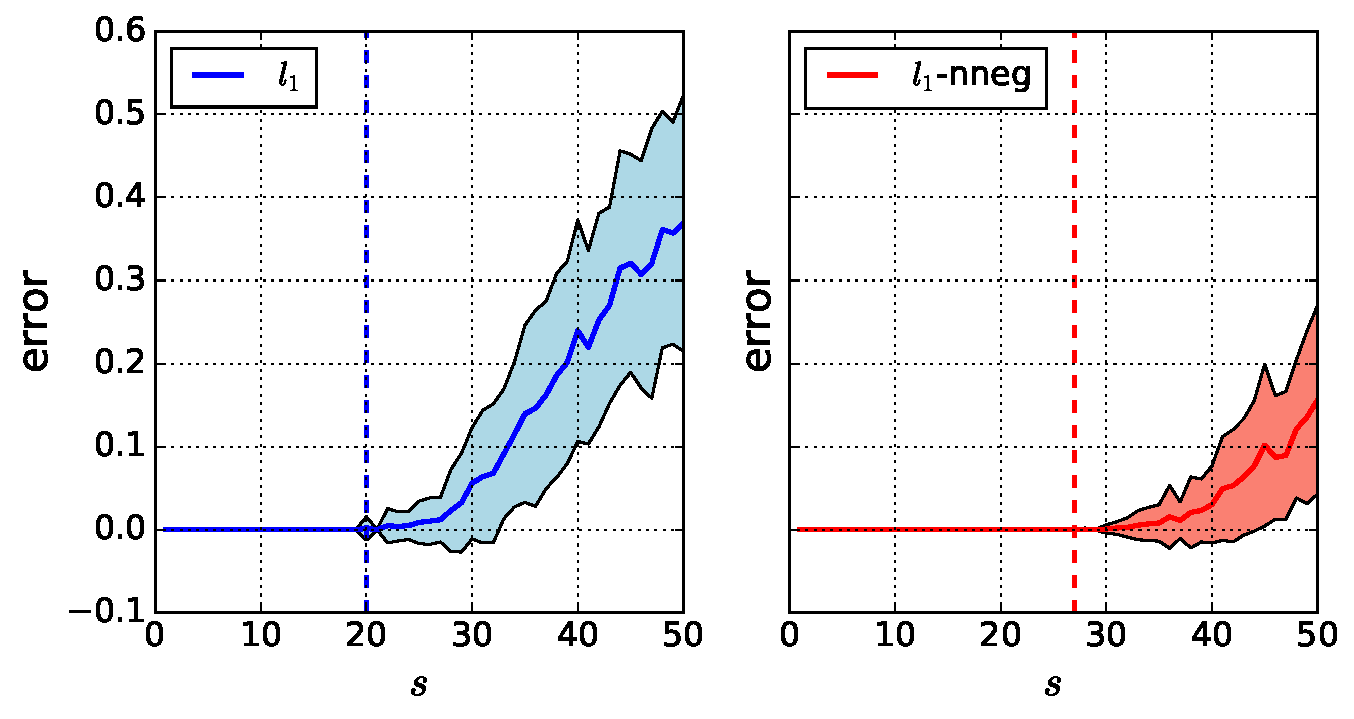
\includegraphics[width=0.7\columnwidth]{figs/error.pdf}
        \caption{The mean and standard deviation of the error for the
        $l1$-minimizaion problem (left) and the $l1$-non-negative-minimizaion
        problem (right).}
        \label{fig:error}
      \end{figure}
      
      The python code for this simulation is as follows:

    }
\begin{lstlisting}[language=Python]
import numpy as np
import scipy as sp
import cvxpy as cvx

import timeit
import sys
from IPython.display import clear_output

N = 100 # Number of repetition
k = 100
d = 400

s_range = np.arange(1, 51, dtype="int32") # range of s

A = np.random.randn(k, d, N)

err = np.zeros([len(s_range), N], dtype="float64") # The relative error for l1-minimization
err_nn = np.zeros([len(s_range), N], dtype="float64") # The relative error for non-neg l1-minimization

for idx, s in enumerate(s_range):
    X = np.random.randn(s, N)
    err_tmp = np.zeros(N, dtype="float64")
    for n in range(N):
        S = np.random.choice(d, s, replace = False) # Uniformly choose the locations of non-zero elements
        
        x = np.zeros(d, dtype="float64")
        x[S] = X[:, n]
        y = np.dot(A[:, :, n], x)
        z = cvx.Variable(d)
        prob = cvx.Problem(cvx.Minimize(cvx.norm(z, 1)), [A[:, :, n] * z == y,])
        prob.solve()
        err[idx, n] = (np.linalg.norm(z.value.flatten() - x) ** 2) / (np.linalg.norm(x) ** 2)
        
        x = np.zeros(d, dtype="float64")
        x[S] = np.absolute(X[:, n])
        y = np.dot(A[:, :, n], x)
        z = cvx.Variable(d)
        prob = cvx.Problem(cvx.Minimize(cvx.norm(z, 1)), [A[:, :, n] * z == y, z >= 0])
        prob.solve()
        err_nn[idx, n] = (np.linalg.norm(z.value.flatten() - x) ** 2) / (np.linalg.norm(x) ** 2)
        
    #process.stdout
    clear_output()
    print("s={0}, err={1}, err_nn={2}".format(s, err[idx, :].mean(), err_nn[idx, :].mean()))
    sys.stdout.flush()
    
err_mean = err.mean(axis = 1)
err_std = err.std(axis = 1)

err_nn_mean = err_nn.mean(axis = 1)
err_nn_std = err_nn.std(axis = 1)

threshold = 1e-10
idx_nz = np.where(err_mean > threshold)[0].min() # The first non-zero position
idx_nn_nz = np.where(err_nn_mean > threshold)[0].min()

import matplotlib as mpl
import matplotlib.pyplot as plt
%matplotlib inline

axis_font = {'size':'20'}
mpl.rcParams['xtick.labelsize'] = 16
mpl.rcParams['ytick.labelsize'] = 16

fig, axs = plt.subplots(1, 2, sharey=True, sharex=True, figsize=(10, 5))

axs[0].plot(s_range, err_mean, 'blue', linewidth=2, label="$l_1$")
axs[0].fill_between(s_range, err_mean-err_std, err_mean+err_std, facecolor='lightblue')
axs[0].axvline(s_range[idx_nz], color='blue', linestyle='--', linewidth=2)
axs[0].legend(prop={'size':16}, loc=2)
axs[0].grid()
axs[0].set_xlabel('$s$', **axis_font)
axs[0].set_ylabel('error', **axis_font)

axs[1].plot(s_range, err_nn_mean, 'red', linewidth=2, label="$l_1$-nneg")
axs[1].fill_between(s_range, err_nn_mean-err_nn_std, err_nn_mean+err_nn_std, facecolor='salmon')
axs[1].axvline(s_range[idx_nn_nz], color='red', linestyle='--', linewidth=2)
axs[1].legend(prop={'size':16}, loc=2)
axs[1].grid()
axs[1].set_xlabel('$s$', **axis_font)
axs[1].set_ylabel('error', **axis_font)

fig.savefig('error.pdf', dpi=10, bbox_inches='tight')
\end{lstlisting}
  \end{homeworkProblem}
  
  %----------------------------------------------------------------------------------------
  % PROBLEM 5
  %----------------------------------------------------------------------------------------
  \begin{homeworkProblem}
    Same setup as in Problem 4, but now the non-zero entries of $\mathbf{x}$ are
    non-negative. Taking this information into account, we now solve
    \begin{align}
      \min_{\mathbf{z}}\|\mathbf{z}\|_1,\; \mbox{subject to } \mathbf{Az} =
      \mathbf{y}\,\mbox{and}\,\mathbf{z}\geq \mathbf{0}
      \label{eq:l1_nn}
    \end{align}
    (here, $\mathbf{z}\geq \mathbf{0}$ is meant entrywise, i.e., for each $k$:
    $z_k \geq 0$). (The positivity constraint is easy to include in CVX).
    Repeat the simulations as described in Problem 4. Compare your findings to
    the results from your experiments of Problem 4 and try to quantify the
    difference regarding the range for $\mathbf{s}$ for which recovery is still
    possible in this case.
    
    \vspace{10pt}
      
    \problemAnswer{
      See Problem 4.
    }
  \end{homeworkProblem}
  
  %\newpage
  %\begin{appendices} 
  %\end{appendices}
  %$\bibliographystyle{unsrt}
  %\bibliography{refs}
  
  %----------------------------------------------------------------------------------------

\end{document}